\section{Evaluation}
% The experimental results are presented and analyzed in this section.
% In detail, experimental settings are introduced in Sec.~\ref{sec:experiment-settings}.
% Sec.~\ref{sec:experiment-e2e}-Sec.~\ref{sec:experiment-case-study} conduct the end-end experiments, test on queries with cycles, perform ablation studies, evaluate the optimization efficiency, test the efficiency of optimziations accross reltaional and graph queries, and evaluate the efficiency of the join order of the plans generated by \name, respectively.

\begin{table}[t]
    \centering
    \begin{tabular}{c|c|c|c}
    \hline
    Dataset & |V| & |E| & Disk Space Usage\\
    \hline
    $G_{sf10}$& 29,987,835 & 88,317,856 & 8.9G \\
    \hline
    $G_{sf30}$ & 88,789,833 & 278,652,443 & 28.0G\\
    \hline
    $IMDB$ & 14,431,946 & 59,758,241 & 3.7G \\
    \hline
    \end{tabular}
    \caption{Statistics of the datasets. In detail, $|\cdot|$ represents the number of elements in $\cdot$.}
    \label{table:experiment-datasets}
\end{table}

\subsection{Experimental Settings}
\label{sec:experiment-settings}

\noindent\textbf{Benchmarks.} Our experiments leverage two widely used benchmarks to assess system performance, as follows:
\begin{itemize}
    \item \textbf{LDBC SNB.} We follow the Linked Data Benchmark Council (LDBC) social network benchmark~\cite{ldbc_snb} to test the system. We use two commonly-adopted datasets with scale factors of 10 and 30, denoted as $G_{sf10}$ and $G_{sf30}$ respectively, generated by the official LDBC Data Generator.
    We select 10 queries from the LDBC Interactive workload for evaluation, denoted as $IC[1, \ldots, 9, 11, 12]$, with $10$, $13$, and $14$ excluded since they involve either pre-computation or shortest-path that are not supported.
    We slightly modified the queries containing variable-length joins by separating them into several individual queries with a suffix ``$-l$'' denoting the fixed length, as following~\cite{graindb}.
    In addition, we carefully designed two sets of queries for the comprehensiveness of evaluation, including (1) $QR[1\ldots 4]$, comprising four queries to test the effectiveness of heuristic rules \filterrule and \joinfuserule in \name, and (2) $QC[1\ldots 3]$, comprising three typical patterns with cycles including triangle, square, and 4-clique, respectively, to assess the efficiency of the advanced extend-intersect operators introduced in \name.
    \item \textbf{JOB.} The Join Order Benchmark (JOB)~\cite{job_snb} on Internet Movie Database (IMDB) is adopted. We select the variants marked with ``a'' of all JOB queries, referred to as $JOB[1\ldots 33]$, without loss of generality. These queries are primarily designed to test join order optimization, with each query containing an average of $8$ joins.
\end{itemize}
The details of the dataset statistics are summarized in Table \ref{table:experiment-datasets}, and all queries are listed in \todo{a supplementary of the paper}.

\noindent\textbf{Compared Systems. }
To ensure a fair comparison, all the following systems use DuckDB as the underlying relational execution engine, with the exception of the optimizer.

\begin{itemize}
\item DuckDB~\cite{duckdb}: This system optimizes queries using the graph-agnostic optimizer described in \refsec{relational-only}, without utilizing the graph index (\refsec{graph-index}) for query execution. It serves as the naive baseline for extending a relational database system to support \spjm.

\item GrainDB~\cite{duckdb}: This system optimizes queries using the graph-agnostic optimizer from \refsec{relational-only} and employs the graph index for query execution. It acts as the baseline to demonstrate that solely using a graph index is insufficient for optimizing \spjm.

%\item \relgohash: This system optimizes queries using the graph-agnostic optimizer introduced in \refsec{converged}, without leveraging the graph index for query execution. It serves as the baseline to showcase that, even in the absence of a graph index, the converged optimizer can generate efficient plans with improved join orders by utilizing graph-optimization techniques.

\item \name: This system optimizes queries using the graph-agnostic optimizer presented in \refsec{converged} and utilizes the graph index for query execution. It demonstrates the full range of techniques introduced in this paper.
\end{itemize}
%We compare \name against two state-of-art baseline systems: DuckDB~\cite{duckdb} as a representative of $Rel$ optimizers, and GrainDB~\cite{graindb} as a representative of $Rel^+$ optimizers.
%For fair comparison, we use DuckDB as the underlying relational engine for all compared systems.
%To facilitate the evaluation of further optimizations brought by GrainDB and \name,
%we integrate pre-built graph indices into the backend storage, and implement the \intersect~ operator with worst-case optimal join implementation in the backend DuckDB engine.
%In this case, all the plans generated by different optimizers in the compared systems can be executed on the same backend.
%Then the comparison between these systems lies in their optimizers: DuckDB's optimizer will not consider the graph indices in query optimization, such that all queries will be executed with hash joins (even when graph indices are available);
%GrainDB will leverage the graph indices, and replace some hash joins with sip joins or merge sip joins to improve the efficiency of the plans;
%and for \name, in addition to graph indices, it will further consider converged optimizations across graph and relational query semantics, and leverage the optimized implementation for intersect operators.
%For simplicity, in the following, when there is no ambiguity, the optimizers of DuckDB and GrainDB are shortened to DuckDB and GrainDB, respectively.

% We compare \name against two state-of-art baseline systems: DuckDB~\cite{duckdb} as a representative of $Rel$ optimizers, and GrainDB~\cite{graindb} as a representative of $Rel^+$ optimizers.
% For fair comparison, we use the backend of GrainDB, which integrated pre-built graph indices, as a common backend for all compared systems.
% As the latest released GrainDB is based on an old version of DuckDB, which may miss out the latest optimizations developed in DuckDB, we upgrade the integrated DuckDB (in GrainDB) to v0.9.2.
% Meanwhile, when compared with DuckDB, we also use the same version.
% The difference between DuckDB and GrainDB lies in the optimizer, where DuckDB's optimizer will not consider the graph indices in query optimization, such that all queries will be executed with hash joins (even when graph indices are available),
%  while GrainDB will leverage the graph indices, and replace some hash joins with sip joins (or merge sip joins) to improve the efficiency of the plans.
% For \name, we further implement extend-intersect operators in the backend (as discussed in \refsec{physical-operators}), which not only leverage the graph indices, but also has an optimized worst-case optimal join implementation for \intersect.
% Therefore, all the generate plans can be executed on the same backend, and the efficiency of the plans obtained by varied optimizers can be compared fairly.
% Note that codegen techniques can be employed to facilitate the transformation of the physical plans into executable code.
% For simplicity, in the following, when there is no ambiguity, the optimizers of DuckDB and GrainDB are shortened to DuckDB and GrainDB, respectively.

\noindent\textbf{Configurations. }
Our experiments were conducted on a server equipped with an Intel Xeon E5-2682 CPU running at 2.50GHz and 251GB of RAM, with parallelism restricted to a single thread.
%We use the latest version of DuckDB as the common relational execution engine.
%To build the graph indices, we adhered to the same procedures for data processing and graph index construction as outlined in~\cite{graindb}.
%Note that codegen techniques can be employed to facilitate the transformation of the physical plans into executable code.
For a comprehensive performance analysis, each query from the LDBC benchmark was run 50 times using the official parameters, while each query from the JOB benchmark was executed 10 times. We report the average time cost for each query to mitigate potential biases.
We imposed a timeout limit of 10 minutes for each query, and queries that fail to finish within the timeout are marked as \ot.

\subsection{Micro Benchmarks on Optimizers}
\label{sec:experiment-opt}
In this subsection, we conduct three micro benchmarks to evaluate the effectiveness of \name,
including evaluating the optimization efficiency by comparing \name with a volcano optimizer and GrainDB, testing the advanced optimization strategies adopted in \name, and comparing the efficiency of join order optimization between \name, GrainDB, and DuckDB.

\noindent\textbf{Optimization Efficiency Evaluation.}
As we discussed in \refsec{handling-match-operator}, \name is exponentially faster than traditional volcano-style optimizers in optimization cost in theoretical analysis.
To validate this, we designed an experiment to compare the optimization cost of \name against Apache Calcite, which is a widely used data management framework that incorporates a volcano-style query optimizer, with its default optimization rules applied.
Besides measuring the time cost of optimization, we evaluated the execution time for the query plans generated by both \name and Calcite, so as to further evaluate the plan quality.
To ensure a broad comparison, we also included GrainDB in our analysis. Although GrainDB is not a volcano-style optimizer and generally employs a greedy plan optimization approach,
comparing the performance of \name and GrainDB provides insights into whether the optimization time invested by \name is justified.
We omit the results of DuckDB, since its optimization time align with GrainDB, while its execution efficiency generally lags behind GrainDB in most cases.
We select two subsets of the LDBC and JOB queries without loss of generality, and conduct the experiments on $G_{sf30}$ and IMDB datasets respectively.
The results are shown in Fig.~\ref{fig:exp-optimization}.

The experimental results reveal \name is significantly faster in optimization compared to Calcite.
Furthermore, the execution times of the query plans optimized by \name are either faster or comparable to those produced by Calcite.
For example, in the LDBC queries ($IC[7]$ excluded) shown in \reffig{exp-opt-ldbc}, the optimization time cost of \name is about two orders of magnitude faster than that of Calcite, and the execution time of the plans optimized by \name is more than 52.0$\times$ faster, on average.
It is worth noting that for query $IC[7]$ and all queries in JOB, Calcite cannot even finish the optimization within the timeout limit (thus we omit the results of Calcite in \reffig{exp-opt-job}).
On the contrary, \name shows an efficient optimization process for these queries.
This stark contrast accentuates \name's capability to efficiently generate optimized plans, demonstrating its superior optimization performance compared to traditional volcano-style optimizers like Calcite.

Then we move to the comparison between \name with GrainDB. Compared with GrainDB, \name demonstrates a slightly higher optimization cost. This outcome is expected to some extent, given GrainDB's design focuses on greedy, faster optimization methods.
Nevertheless, the quality of \name's optimized plans are usually superior. This can be observed in the execution time results, where \name outperforms GrainDB by $9.5\times$ and $2.8\times$ on average on the $G_{sf30}$ and IMDB datasets, respectively.
For the total time cost of optimization and execution, \name still achieves $6.5\times$ and $2.2\times$ speedup over GrainDB on average, on the $G_{sf30}$ and IMDB datasets, respectively.
%This gap could be more obvious when the dataset scales up (comparing $G_{sf10}$ and $G_{sf30}$), since the optimization time cost is fixed, but a better plan will achieve more efficiency when the dataset scales up.
These findings suggest that \name's optimization cost is justified, as it generates high-quality plans that are more efficient than those optimized by GrainDB in execution.
To ensure a fair comparison, in the subsequent experiments, we evaluate the efficiency of different systems by considering the total time for both optimization and execution.

\todo{\reffig{exp-opt-ldbc} has a log scale on the y-axis, which may not be a good idea?}

\begin{figure}[ht]
    \centering
    \begin{subfigure}[b]{0.45\linewidth}
        \centering
        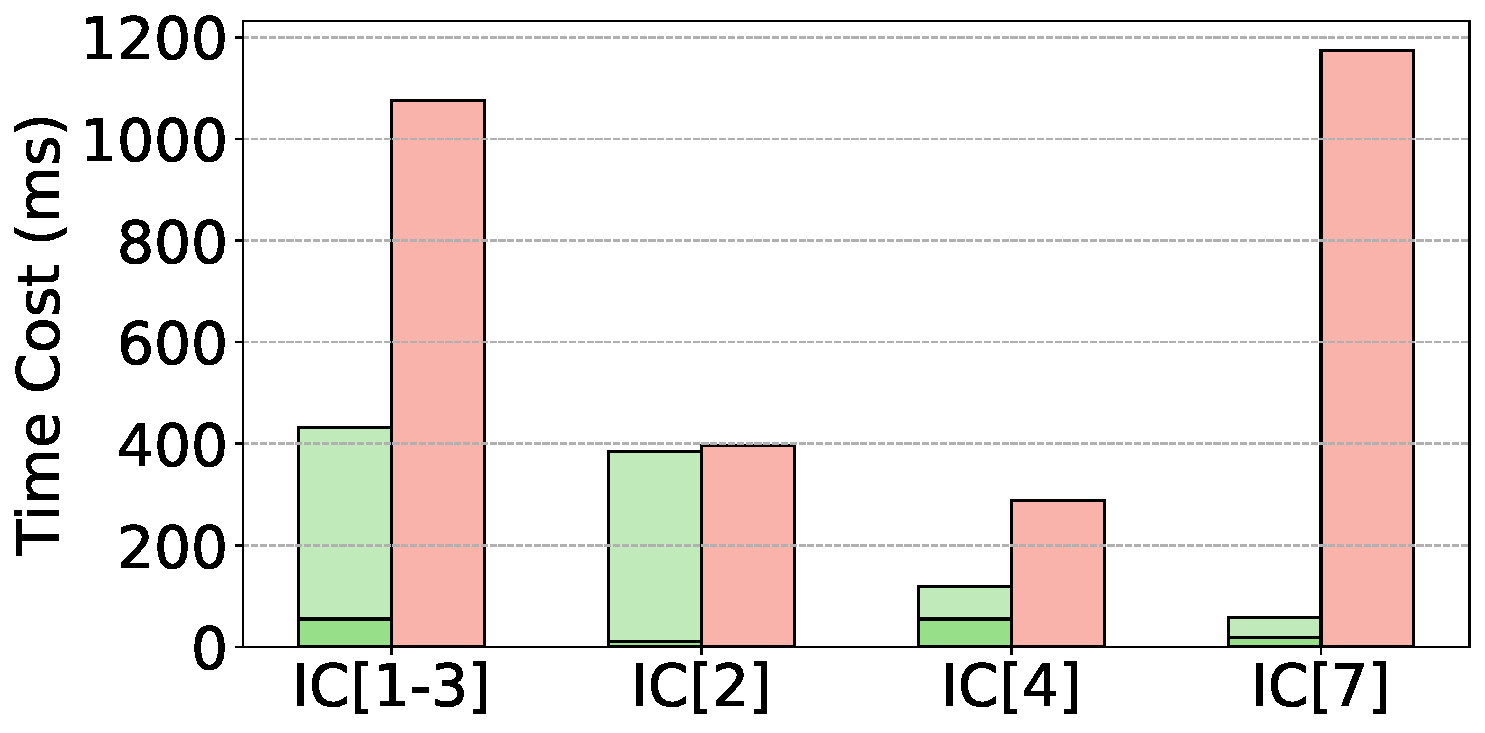
\includegraphics[width=\linewidth]{./figures/exp/opt_exe_ldbc.pdf}
        \caption{Opt. and Exe. Time on $G_{sf30}$.}
        \label{fig:exp-opt-ldbc}
    \end{subfigure}
    \begin{subfigure}[b]{0.45\linewidth}
        \centering
        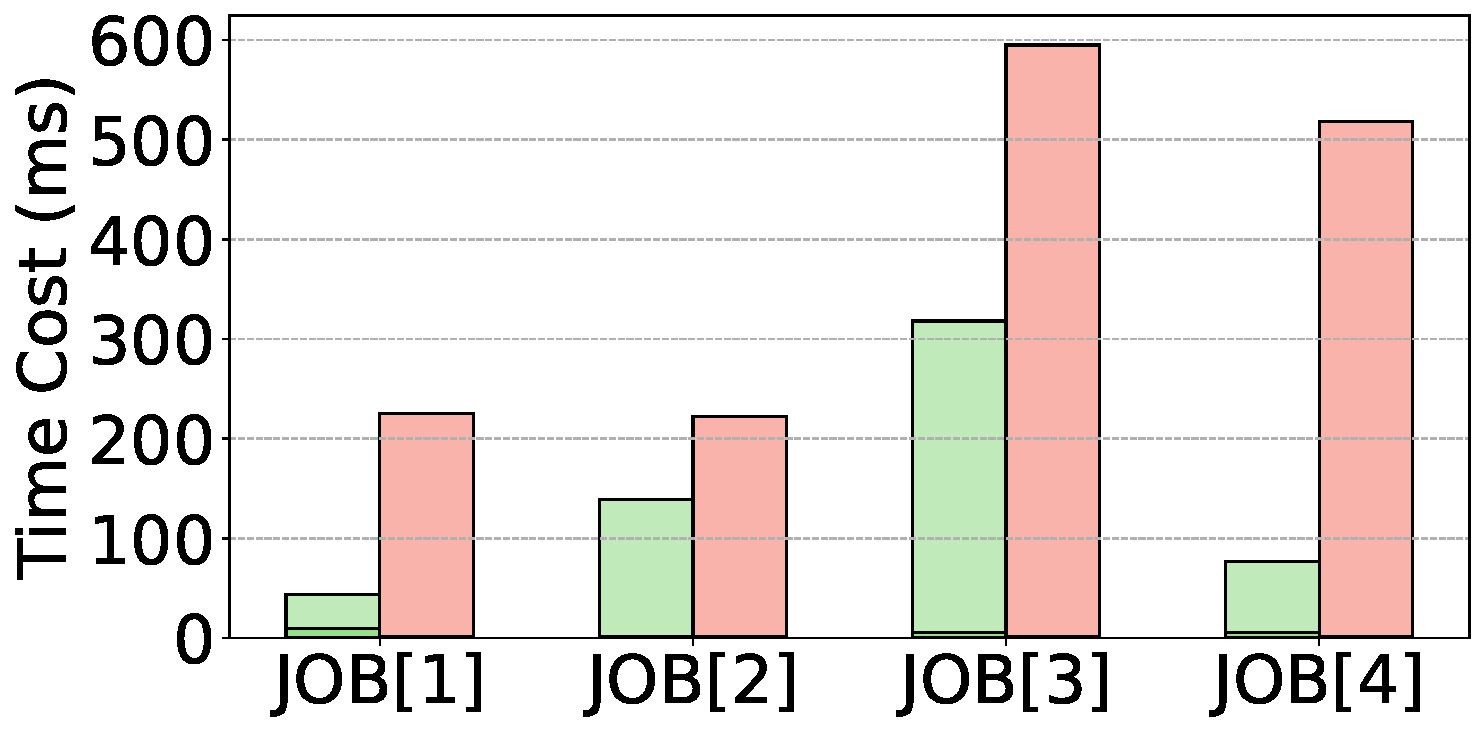
\includegraphics[width=\linewidth]{./figures/exp/opt_exe_job.pdf}
        \caption{Opt. and Exe. Time on IMDB.}
        \label{fig:exp-opt-job}
    \end{subfigure}
    \caption{Experiments on Optimization and Execution Cost}
    \label{fig:exp-optimization}
\end{figure}

% In the experiments, optimizing all the queries with \name can be finished in 10 minutes, while optimizing some queries with Calcite exceeds the 10-minute limit.
% For example, when JOB benchmark is utilized, the time cost of optimizing all the queries with Calcite is longer than 10 minutes.
% As shown in Fig.~\ref{fig:exp-optimization}, \name is much more efficient than Calcite in optimizing queries, and it is consistent with the conclusions obtained in Sec.~\ref{sec:theoretical-analysis}.
% That is, \name is exponentially faster than Calcite in query optimization.
% For instance, when IC5-1 is queried on $G_{sf30}$, the time cost of query optimization with \name can be more than $10^4\times$ faster than that of Calcite.

% Besides, the optimization time cost of \name is similar on $G_{sf10}$ and $G_{sf30}$, and so is Calcite.
% The reason is that the time required for optimization is not significantly associated with the scale of the dataset; instead, it is related to the relative cardinalities among the different tables.
% The relative cardinalities in LDBC datasets of different scales are consistent, therefore the optimization time is similar.

\begin{figure}[ht]
    \centering
    \begin{subfigure}[b]{.45\linewidth}
        \centering
        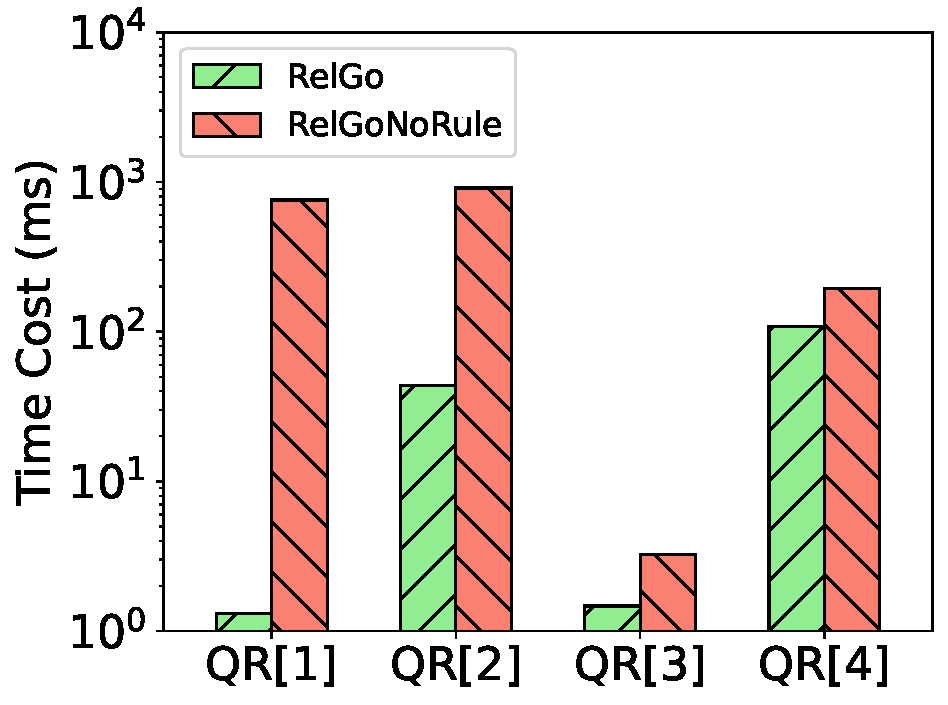
\includegraphics[width=\linewidth]{./figures/exp/filter_sf10.pdf}
        \caption{Time Cost on $G_{sf10}$.}
        \label{fig:exp-filter-sf10}
    \end{subfigure}
    \begin{subfigure}[b]{0.45\linewidth}
        \centering
        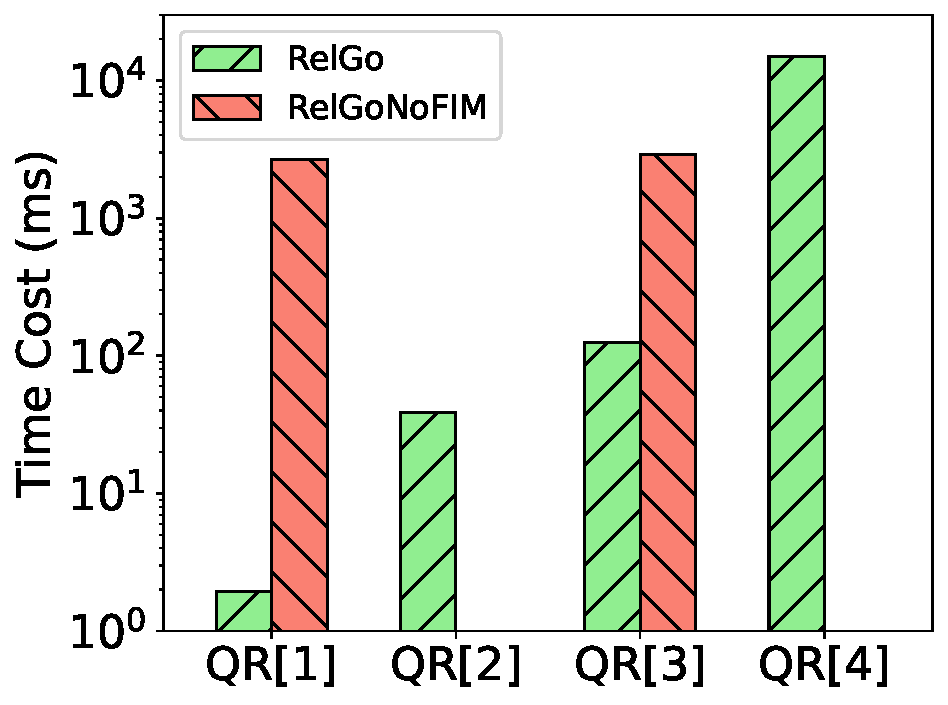
\includegraphics[width=\linewidth]{./figures/exp/filter_sf30.pdf}
        \caption{Time Cost on $G_{sf30}$.}
        \label{fig:exp-filter-sf30}
    \end{subfigure}
    \caption{Efficiency Comparison of \name and \relgonofi}
    \label{fig:exp-filter}
\end{figure}

\begin{figure}[ht]
    \centering
    \begin{subfigure}[b]{.45\linewidth}
        \centering
        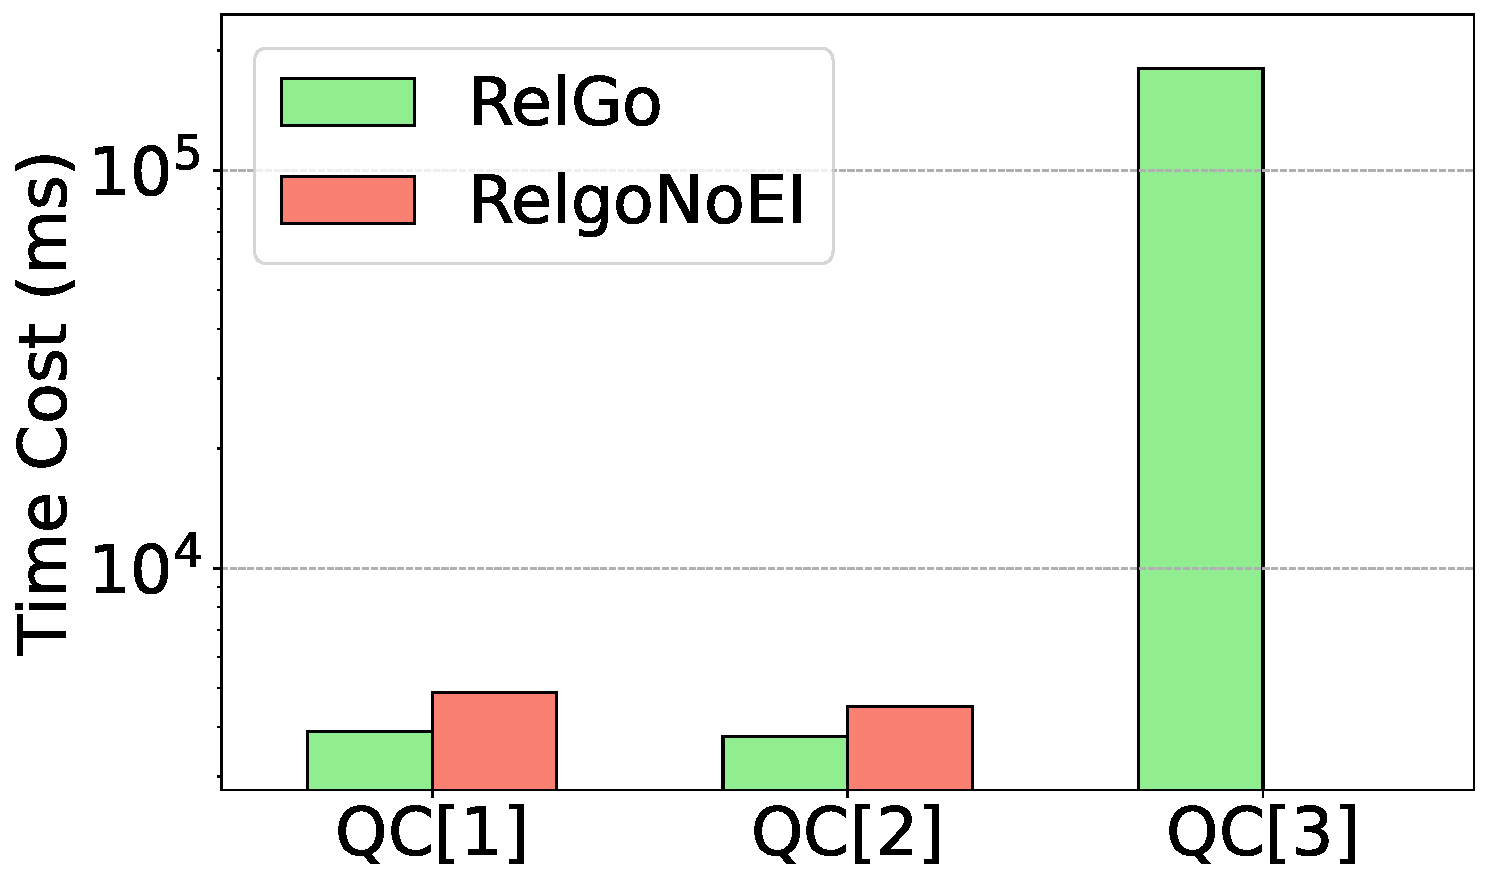
\includegraphics[width=\linewidth]{./figures/exp/ablation_ei_sf10.pdf}
        \caption{Time Cost on $G_{sf10}$.}
        \label{fig:exp-expand-intersect-sf10}
    \end{subfigure}
    \begin{subfigure}[b]{0.45\linewidth}
        \centering
        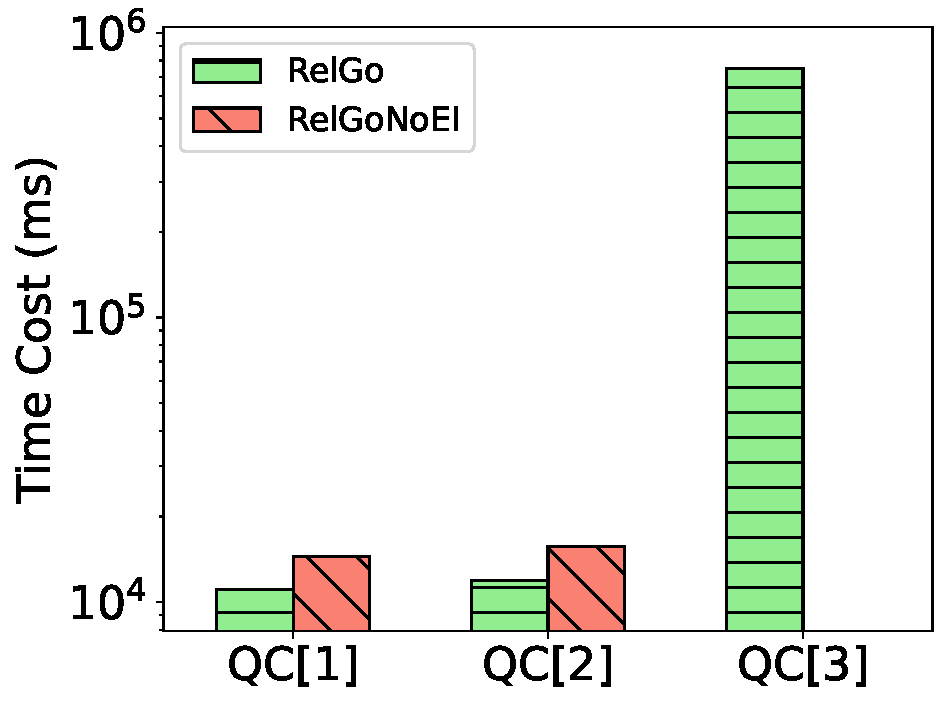
\includegraphics[width=\linewidth]{./figures/exp/ablation_ei_sf30.pdf}
        \caption{Time Cost on $G_{sf30}$.}
        \label{fig:exp-expand-intersect-sf30}
    \end{subfigure}
    \caption{Efficiency Comparison of \name and \relgomj}
    \label{fig:exp-expand-intersect}
\end{figure}

\noindent\textbf{Advanced Optimization Strategies.}
We introduced several advanced optimization strategies in \name, such as the heuristic rules \filterrule and \joinfuserule, and optimized implementation of \expandintersectrule used in cost-based optimizations.
In this experiment, our primary objective is to assess the impact and effectiveness of these optimization strategies.

First we test the \filterrule and \joinfuserule, which are two of the most representative heuristic rules employed in \name that captures the optimization opportunities at the interplay of relational and graph optimizations.
We conduct experiments of $QR[1\dots 4]$ on $G_{sf10}$ and $G_{sf30}$, with $QR[1]$ and $QR[2]$ to evaluate the \filterrule, and $QR[3]$ and $QR[4]$ to assess the \joinfuserule.
The results are depicted in \reffig{exp-filter}, where \relgonofi denotes the variants of \name without corresponding rules.
According to the results, \filterrule~ demonstrates a significant improvement in query performance, with an average speedup of 299.4$\times$ and 699.8$\times$ on $G_{sf10}$ and $G_{sf30}$, respectively.
The \joinfuserule also accelerates the query execution by 2.0$\times$ and 2.3$\times$ on average on $G_{sf10}$ and $G_{sf30}$, respectively.
These results suggest that the heuristic rules, especially the \filterrule, are effective in enhancing the efficiency of query execution by identifying and exploiting optimization opportunities across relational and graph queries.

Then we evaluate the \expandintersectrule, which is utilized in \name's cost-based optimizations, focusing on improving the efficiency of cyclic patterns by employing a worst-case optimal join implementation.
To this end, we conduct experiments on queries $QC[1\ldots 3]$, which are queries containing cycles, and compare the performance of \name with and without \expandintersectrule.
Note that when \expandintersectrule~ is not applied, the \intersect~ operators in the plans would be replaced with multiple join operators, and this variant is denoted as \relgomj.
The performance results depicted in \reffig{exp-expand-intersect} suggest that, compared to \relgomj, \name achieves a speedup of 1.22$\times$ and 1.31$\times$ on average (QC[3] excluded) on $G_{sf10}$ and $G_{sf30}$, respectively.
% improve the performance of $QC[1]$ and $QC[2]$ by $20.0\%$, and  by $15.7\%$ on $G_{sf10}$, and $23.5\%$ and $24.2\%$ on $G_{sf30}$, respectively.
Notably, for $QC[3]$, which is a complex 4-clique, the plans optimized by \relgomj have an excessive memory overhead and cause an OOM error.
The reason is that applying worst-case optimal joins will generate much fewer intermediate results than applying multiple joins, since numerous results that will not appear in the intersection are prematurely deleted.
The results of this experiment indicate that \expandintersectrule~ can not only significantly enhance query performance, but also reduce spatial overhead to a large extent.

\begin{figure}[ht]
    \centering
    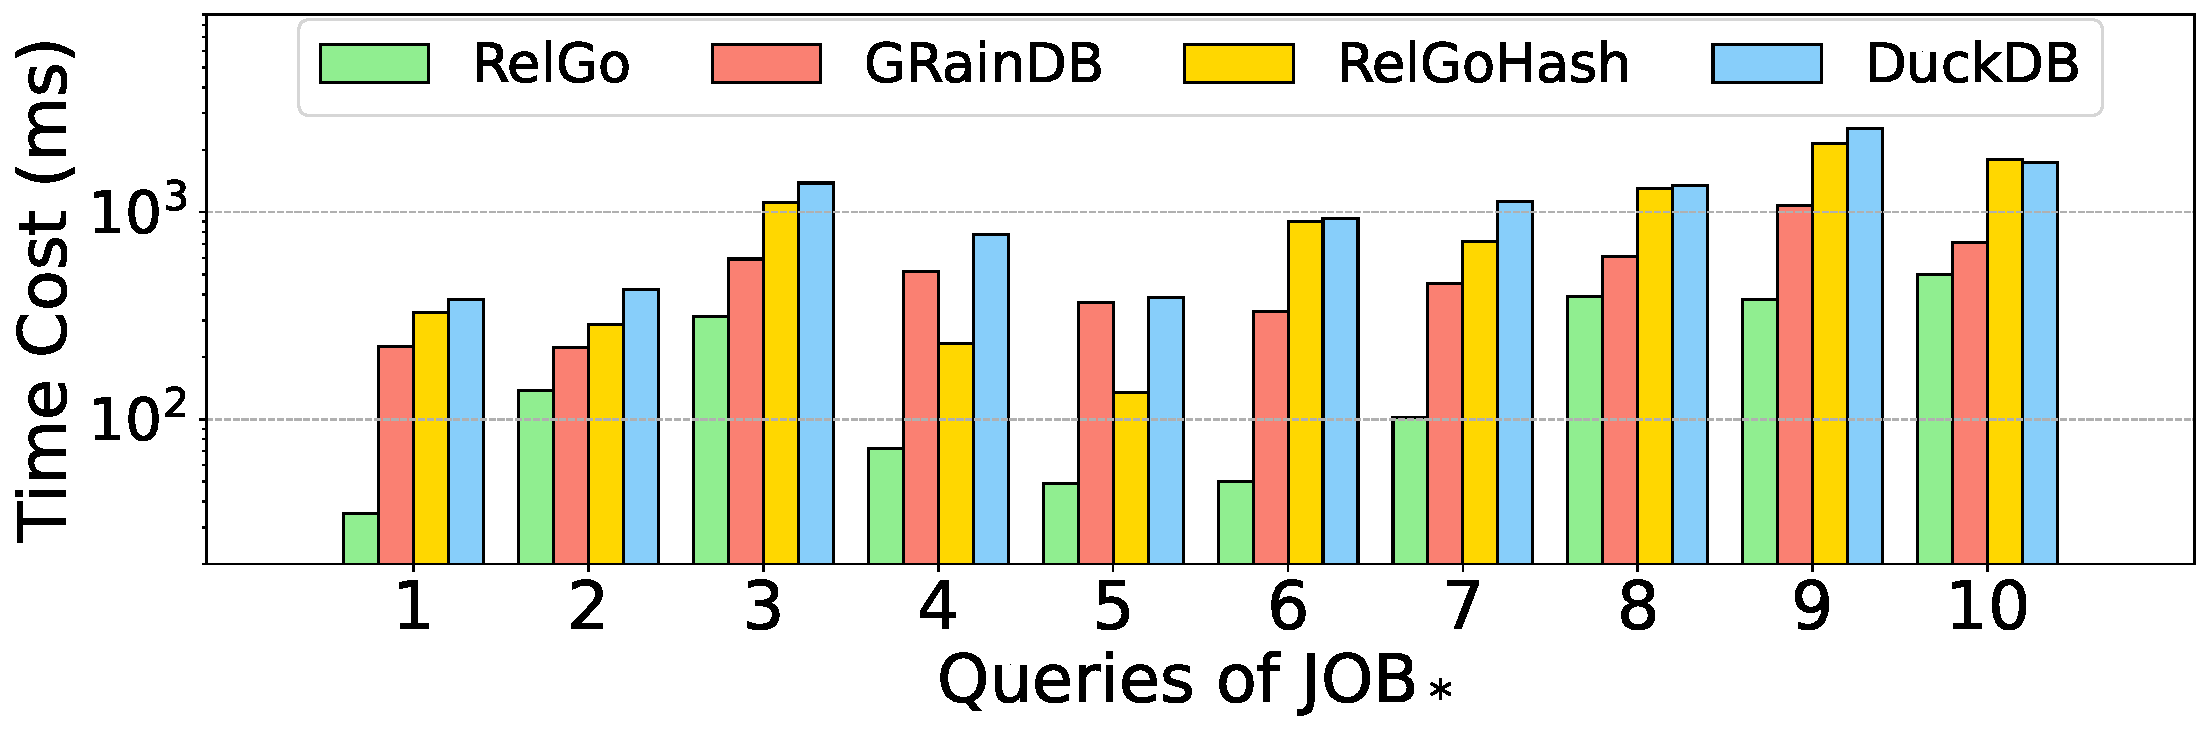
\includegraphics[width=.9\linewidth]{./figures/exp/hash_plan_job.pdf}
    \caption{Efficiency Comparison of \name and Baselines}
    \label{fig:exp-hash-plan}
\end{figure}

\noindent\textbf{Efficiency of Join Order.}
After the assessment of advanced strategies within \name, we integrate all these strategies (and so as in the following experiments) to conduct a performance comparison between \name, \relgohash, GrainDB, and DuckDB with a focus on the join order efficiency.
For this purpose, the JOB benchmark is employed, and without loss of generality, we select queries $JOB[1\ldots 10]$ as representatives.
%Specifically, in addition to the standard \name approach, we further introduce a variant named \relgohash, which exclusively utilizes hash joins for the \expand operations, deliberately bypassing the graph indices to facilitate a more fair comparison with DuckDB.
The performance results are illustrated in Fig.~\ref{fig:exp-hash-plan}.
From the results, we can observe that \name outperforms GrainDB on all the queries, accelerating the execution time from $1.2\times$ to $7.5\times$, and the average speedup is $3.31\times$.
Besides, the plans optimized with \relgohash are always not inferior to those optimized by DuckDB as well, which achieves an average speedup of $1.4\times$, suggesting that even if graph indices are not applied in execution, the join order optimized by \name are still efficient in most cases.
% It is noteworthy that for queries $JOB[4]$ and $JOB[5]$, the execution time of the plans generated by \relgohash is even shorter than those produced by GrainDB,
% It is important to highlight that while graph indices are employed in executing GrainDB's plans, they are not utilized with \name-hash's plans.
It should be noted that \name does not always generate plans featuring the absolute best join orders, since it relies on the estimated cost of the plans.
However, its optimized plans generally remain competitive across a majority of cases, thanks to its integration of high-order statistics that contribute to more accurate cost estimation.
%This superior join order offsets the absence of graph indices in the execution process.


% In this section, we conduct ablation study to show the efficiency of \expandintersectrule.
% In detail, patterns in Fig.~\ref{fig:exp-hard-patterns} are queried on $G_{sf10}$ and $G_{sf30}$, and plans are optimized with Relgo.
% For each plan optimized by Relgo, we replace the extend-intersect operators in it with multiple join operators and obtain a new plan.
% These new plans are called obtained with \textit{"Relgo w.o. EI"}.
% The experimental results are shown in Fig.~\ref{fig:exp-ablation-ei}.

% The results illustrate the efficiency of \expandintersectrule.
% When triangles are searched for, removing the extend-intersect operators decreases the query performance.
% Besides, when butterflies and 4-cliques are searched for, the plans without extend-intersect operators have an excessive memory overhead and cause an ``Out of Memory'' (abbr.~OOM) error.
% The reason is that applying extend-intersect operators has much fewer intermediate results than applying multiple joins, since numerous results that will not appear in the intersection are prematurely deleted.
% It indicates that \expandintersectrule can not only enhance query performance, but also reduce spatial overhead.

% To further demonstrate the efficiency of \expandintersectrule, we add predicates on butterflies (i.e., Fig.~\ref{fig:exp-hard-butterfly}) and 4-cliques (i.e., Fig.~\ref{fig:exp-hard-clique}) to avoid OOM, and generate two new patterns, i.e., \textit{Butterfly-P} and \textit{4-Clique-P}.
% Specifically, for these two new patterns, the values of properties Person1.\textit{p\_personid} are constrained to be smaller than specified values.
% Queries of these new patterns are optimized with GrainDB, \name, and \textit{\name w.r. EI}.
% The results on the constrained-patterns are shown in Fig.~\ref{fig:exp-ablation-para-ei}.


% The results suggest that \expandintersectrule is crucial in optimizing queries with cycles.
% Specifically, for the new patterns with cycles, the execution time of plans optimized by \name is more than an order of magnitude shorter than those optimized by \textit{"Relgo w.o. EI"}.
% It indicates the effectiveness of \expandintersectrule.
% Moreover, when patterns with many cycles are used (e.g., 4-clique in Fig.~\ref{fig:exp-hard-clique}), the optimization effect of the rule becomes particularly noticeable.
% In detail, querying for 4-cliques with \name can be 100$\times$ faster than with \textit{"Relgo w.o. EI"}.
% The results illustrate the efficiency of \expandintersectrule.

\begin{figure*}[ht]
    \centering
    \begin{subfigure}[b]{0.45\linewidth}
        \centering
        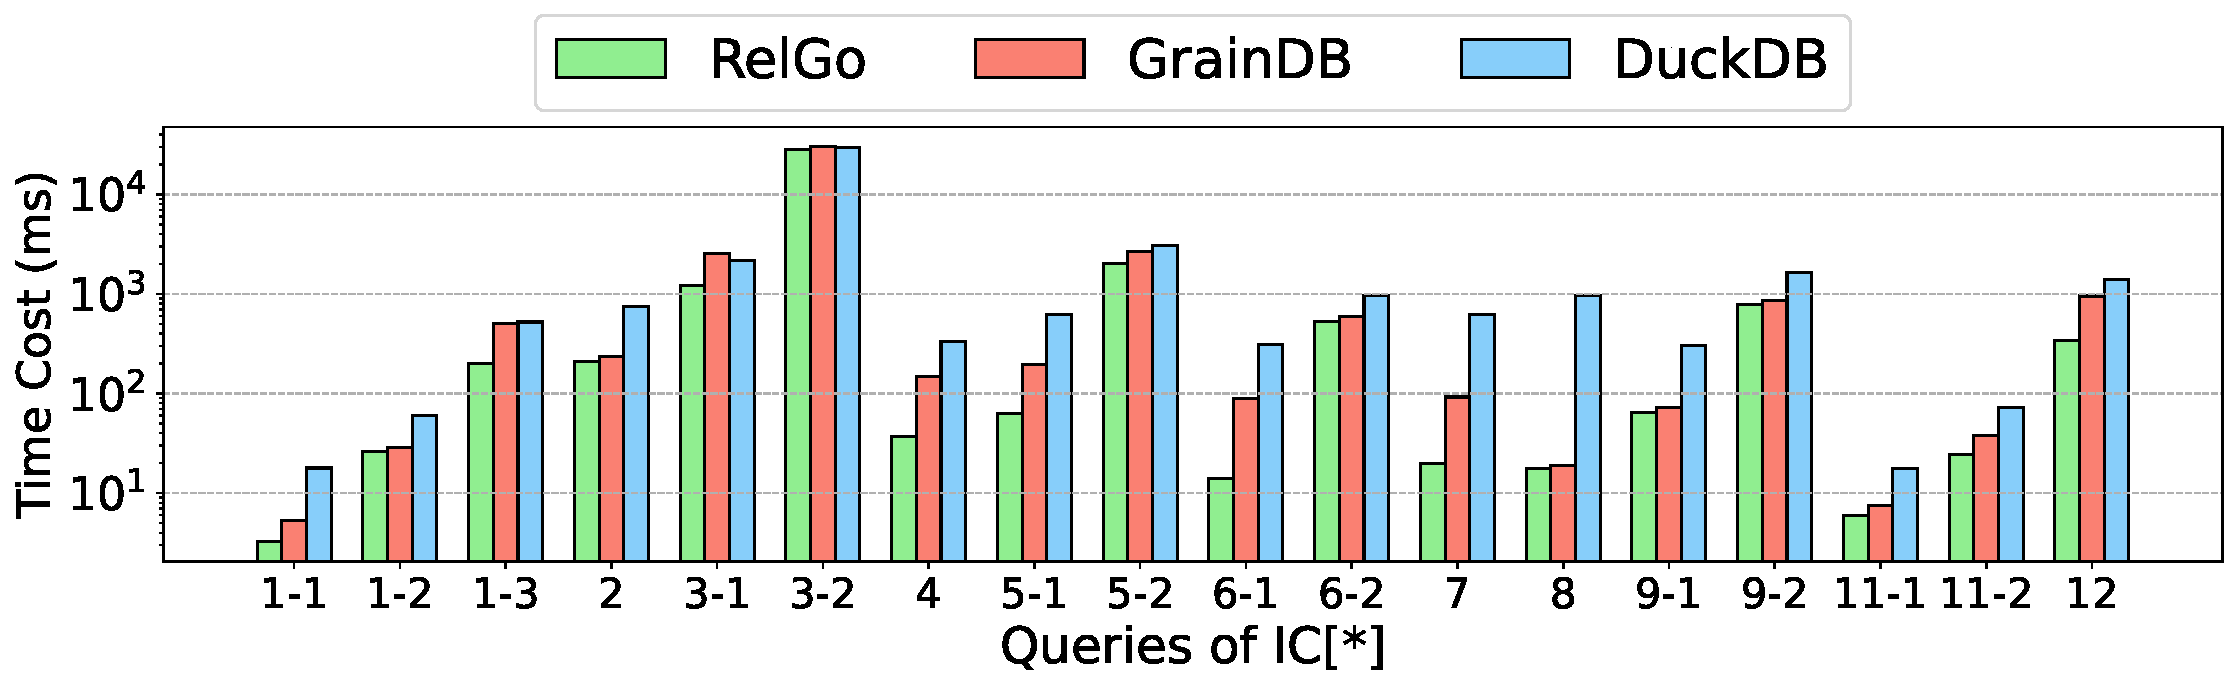
\includegraphics[width=\linewidth]{./figures/exp/e2e_sf10.pdf}
        \caption{Time Cost on $G_{sf10}$.}
        \label{fig:exp-e2e-sf10}
    \end{subfigure}
    \begin{subfigure}[b]{0.45\linewidth}
        \centering
        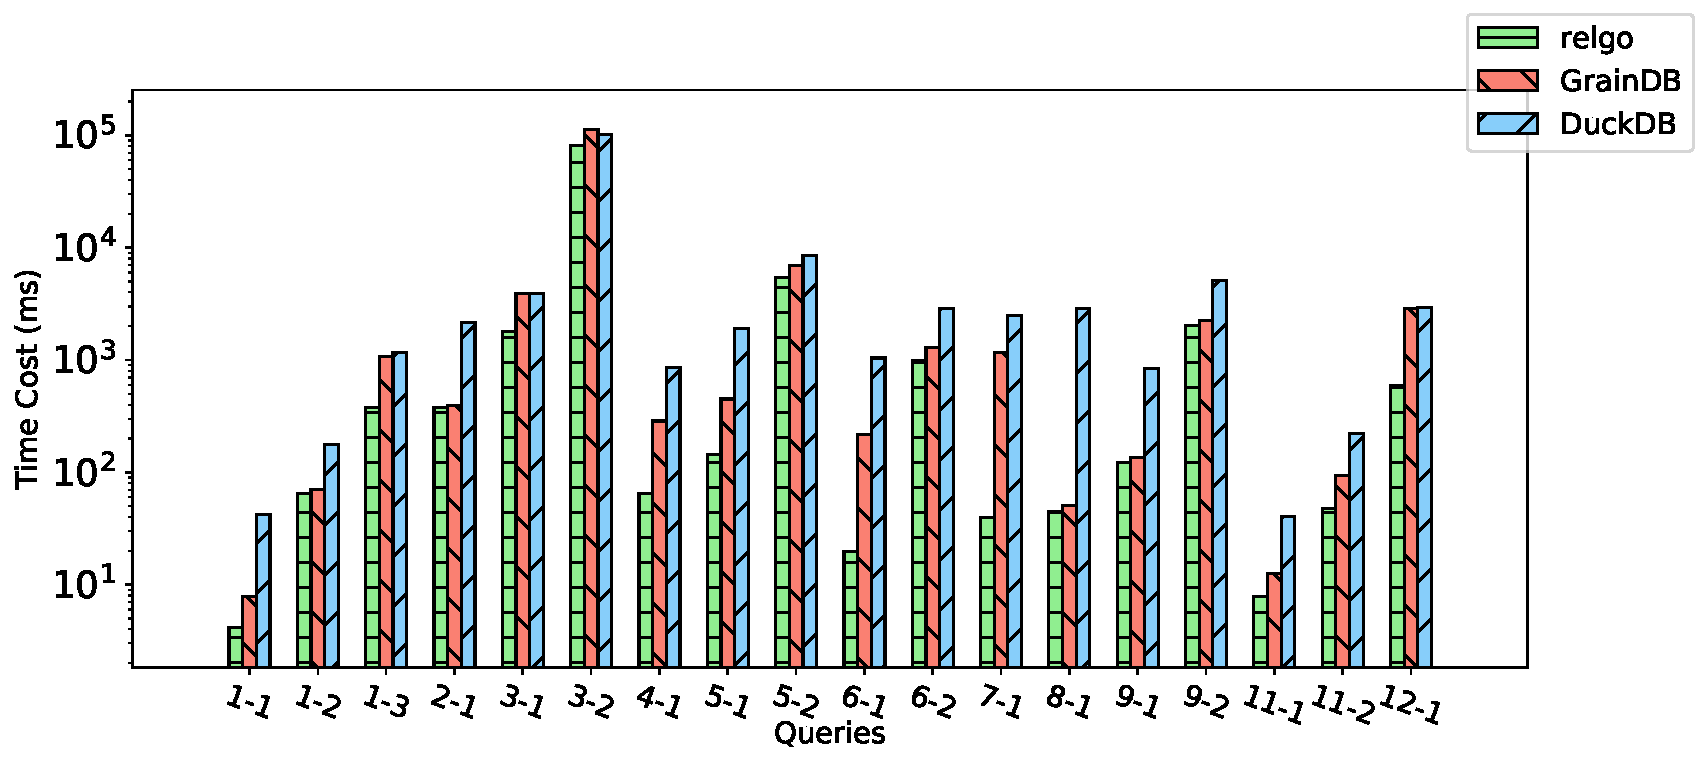
\includegraphics[width=\linewidth]{./figures/exp/e2e_sf30.pdf}
        \caption{Time Cost on $G_{sf30}$.}
        \label{fig:exp-e2e-sf30}
    \end{subfigure}
    \begin{subfigure}[b]{0.6\linewidth}
        \centering
        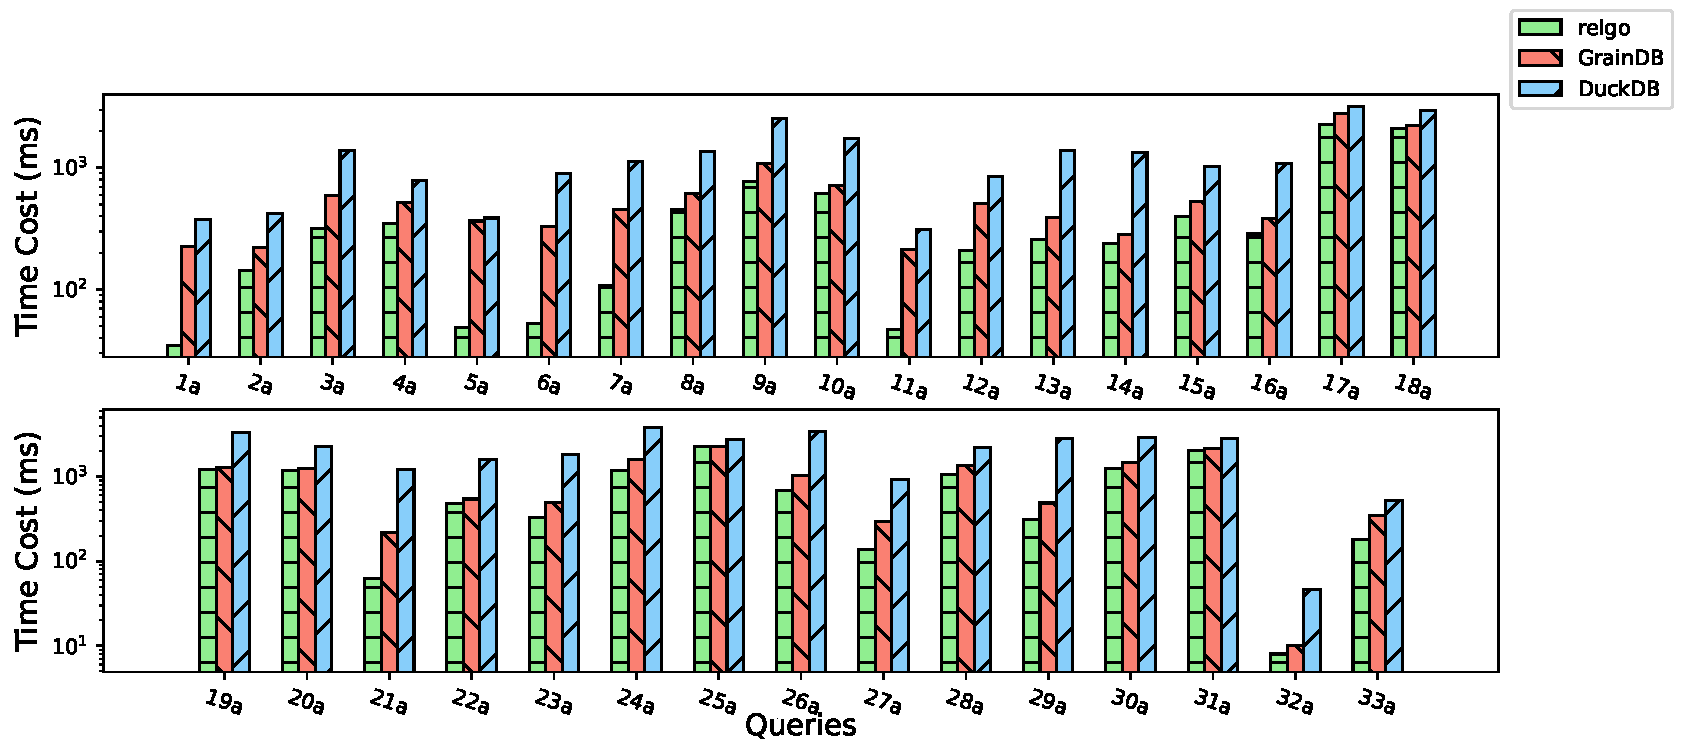
\includegraphics[width=\linewidth]{./figures/exp/e2e_job.pdf}
        \caption{Time Cost on IMDB.}
        \label{fig:exp-e2e-job}
    \end{subfigure}
    \caption{Results of the end-to-end experiments.}
    \label{fig:exp-e2e}
\end{figure*}

\subsection{End-to-End Experiments}
\label{sec:experiment-e2e}

End-to-end experiments are conducted on LDBC and JOB benchmarks for a comprehensive evaluation of the performance of \name compared to GrainDB and DuckDB,
and the experimental results are presented in Fig.~\ref{fig:exp-e2e}.
The results demonstrate that execution plans optimized by \name consistently outperform those optimized by GrainDB or DuckDB on both the LDBC and JOB benchmarks.
Specifically, for the LDBC benchmark, the execution time of the plans optimized by \name is about 2.2$\times$ and 9.1$\times$ faster on average than those generated by GrainDB and DuckDB on $G_{sf10}$, respectively, and about 4.10$\times$ and 14.72$\times$ faster on $G_{sf30}$.
For the JOB benchmark, \name has also achieved better performance compared to GrainDB and DuckDB, with an average speedup of 2.1$\times$ and 5.1$\times$, respectively.

There are mainly three reasons for the superiority of \name.
Firstly, by incorporating a matching operator in \spjm queries to capture the graph query semantics, \name is able to leverage the advanced graph optimization techniques to optimize the matching operator, such as using the high-order statistics to estimate the cost of the plans more accurately, and leveraging the worst-case optimal join implementation to optimize the cyclic patterns.
Conversely, DuckDB and GrainDB cannot benefit from these graph-specific optimizations, and may generate suboptimal plans and have inefficient execution.
%which, for example, rely on low-order statistics that may lead to inaccurate cost estimation, and traditional multiple join implementations for cyclic patterns that are usually inefficient and cannot guarantee worst-case optimal.
Secondly, \name takes the optimization opportunities across the graph and relational query semantics into consideration, introducing effective heuristic rules such as \filterrule and \joinfuserule, which can significantly improve the efficiency of the plans.
Thirdly, without loss of generality, \name is also aware of the existence of graph indices in graph query optimization, and leverages the graph indices to get neighbors of vertices effectively.
On the contrary, GrainDB occasionally partitions this process into separate stages, first retrieving adjacent edges and subsequently obtaining the corresponding endpoints, which may lead to inefficiency in execution. And DuckDB does not consider the graph indices in query optimization, and would execute the queries with hash joins which are not efficient in most cases.

% There are mainly two reasons for the superiority of \name.
% Firstly, \name is aware of the existence of graph indices in graph query optimization.
% Thus, the cost estimation of \name is more accurate and better physical plans can be obtained.
% In contrast, the optimizers of DuckDB and GrainDB are of the types $Rel$ and $Rel^+$, respectively, and are not aware of the graph indices in query optimization phase.
% Therefore, the accuracy of cost estimation is limited.
% Secondly, for queries with cycles (e.g., $IC[7]-1$ on LDBC), \name have a superior performance due to the advanced extend-intersect operators, which outperforms the traditional multiple join operators used by DuckDB and GrainDB.
% Such an operator can significantly reduce the time consumption, which is also demonstrated through experiments in \reffig{exp-expand-intersect}.
% \todo{update this, with the new TrimFusionRule:} Thirdly, \name is more adept at identifying opportunities to effectively utilize graph indices to get neighbors of vertices, since it optimizes graph queries from the graph perspective.
% Conversely, GrainDB occasionally partitions the process into separate stages, first retrieving adjacent edges and subsequently obtaining the corresponding endpoints.
